\section{Syntax highlighting in state panel}
\label{section:state-panel}
This feature was used as starting point to get to know the codebase. The \emph{State Panel} is one of the features which was ported from jEdit by \citeauthor{ivsc_report} when the Isabelle/VSCode extension was first developed. The main purpose of the state panel is to show the internal proof state. The user can update the proof state by either clicking the Update State button or by enabling Auto Update, which then updates the proof state according to the current cursor position in the editor. Being able to preview the proof state is crucial to having an overall better user experience.

The jEdit state panel has syntax highlighting, which matches that of the code editor, shown in \autoref{fig:jedit_state_panel}. On the other hand the VSCode state panel has no syntax highlighting and it is also missing clickable items, as shown in \autoref{fig:vscode_state_panel_before}. This is problematic for user who are accustomed to working with these features.

\begin{figure}[htpb]
  \centering
  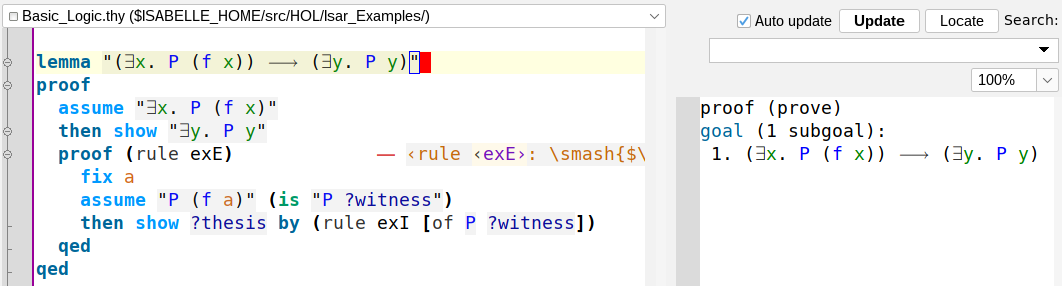
\includegraphics[width=0.8\textwidth]{figures/problem1/jedit_state_panel.png}
  \caption{State panel in jEdit, with the state taken at the current cursor position} \label{fig:jedit_state_panel}
\end{figure}

\begin{figure}[htpb]
  \centering
  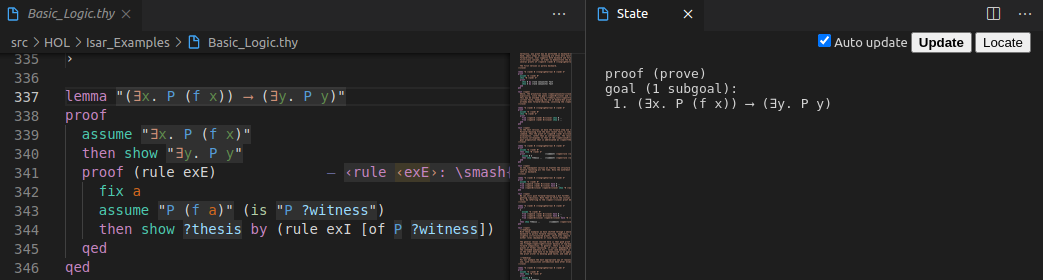
\includegraphics[width=0.8\textwidth]{figures/problem1/vscode_state_panel_before.png}
  \caption{VSCode state panel missing syntax highlighting and clickable items.} 
  \label{fig:vscode_state_panel_before}
\end{figure}

\paragraph{Current implementation.}
In VSCode, the state panel is implemented as a \emph{Webview}, which opens up as a column separately from the active editor. A message is then sent to the language server to show the proof state for the active document for the line in which the cursor is. The language server performs a query to get the state and then replies with a HTML document which is inserted directly into the Webview, in the frontend.

\paragraph{Solutions}
In the current implementation, the server sends to the state panel HTML which has the proper markup to highlight its body, but the body is inserted without markup. The most obvious solution would be to just insert the body with the markup, as shown in \autoref{fig:vscode_state_panel_mid}.
 
\begin{figure}[htpb]
    \centering
    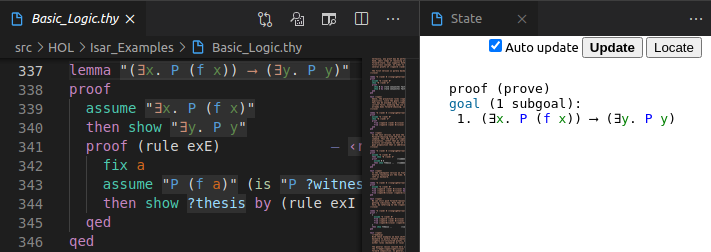
\includegraphics[width=0.8\textwidth]{figures/problem1/vscode_state_panel_mid.png}
    \caption{VSCode state panel with proper markup} \label{fig:vscode_state_panel_mid}
\end{figure}

Even though this is an easy solution and aligns perfectly with how it behaves in jEdit, it is clear that that it does not fit VSCode. The syntax highlighting does not match that of VSCode and most VSCode extensions require support for the dark theme because it is the default and by far the most popular theme.
Another problem with this solution is that we build the whole HTML in the backend, which is not optimal since we have a frontend and our GUI elements seem out of place in VSCode.

The second approach would be to build the HTML for the Webview in the frontend and only ask the backend for the marked-up body. The marked-up body is obtained using the Isabelle HTML presentation elements. Then, the syntax highlighting, which is configured in the settings, is applied to marked-up body. Since the controls are now in the frontend, the state of the auto update checkbox also needs to be correctly set. Now, every update of the state panel comes with the \texttt{id}, the \texttt{auto\_update boolean}, and the \texttt{body} as a \texttt{string}.

The \emph{Output Panel}, which had the same issue, is also given the same treatment as the state panel. The only difference being that the output panel doesn't have controls (Update, Auto-Update, Locate) and is connected with the back-end through another endpoint. 

\paragraph{Results}
The state panel has now syntax highlighting and clickable items. Aside from that it also matches the syntax highlighting to the currently active theme, as shown in \autoref{fig:vscode_state_panel_end}. An advantage of this implementation is that it has a higher degree of decoupling between the backend and the frontend. Also the styling of the GUI elements is consistent.
% \begin{figure}[htbp]
%     \centering
%     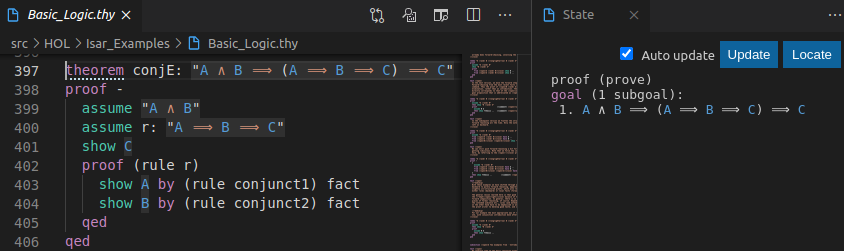
\includegraphics[width=0.8\textwidth]{figures/problem1/vscode_state_panel_end_dark.png}
%     \caption{Dark theme example} \label{fig:vscode_state_panel_end_dark}
% \end{figure}

% \begin{figure}[htbp]
%     \centering
%     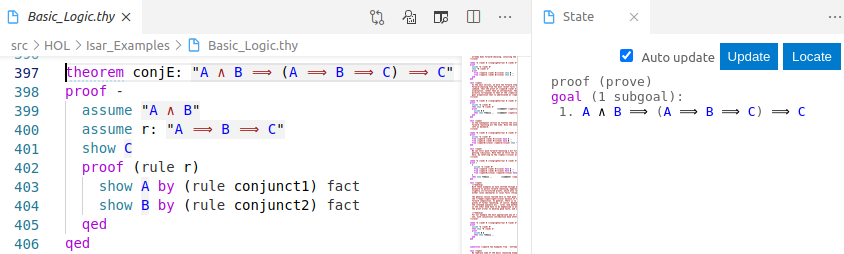
\includegraphics[width=0.8\textwidth]{figures/problem1/vscode_state_panel_end_light.png}
%     \caption{Light theme example} \label{fig:vscode_state_panel_end_light}
% \end{figure}

\begin{figure}[!htbp]
  \centering
  \subfloat[Dark theme][State panel in dark theme.]{
      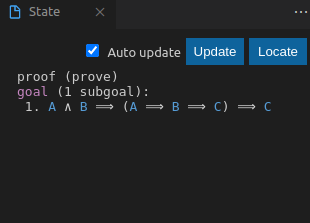
\includegraphics[width=0.45\textwidth]{figures/problem1/vscode_state_panel_end_dark_crop.png}
      \label{fig:vscode_state_panel_end_dark}
  }
  \hfill
  \subfloat[Light theme][State panel in light theme.]{
      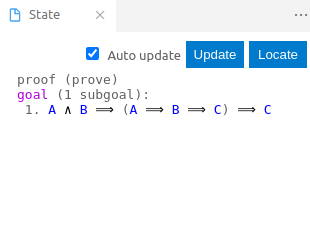
\includegraphics[width=0.45\textwidth]{figures/problem1/vscode_state_panel_end_light_crop.png}
      \label{fig:vscode_state_panel_end_light}
  }
  \caption{VSCode state panel with theme appropriate markup.}
  \label{fig:vscode_state_panel_end}
\end{figure}